\documentclass{article}
\usepackage{fullpage}
\usepackage{graphicx} % Required for inserting images
\usepackage[section]{placeins}
\usepackage{float}
\usepackage{amsmath}
\usepackage{url}
\usepackage{enumitem}

% ABNF listings
\usepackage[utf8]{inputenc} % Use UTF-8 encoding for modern Unicode handling
\usepackage{listings}
\lstset{
    basicstyle=\ttfamily,
    breaklines=true,
    breakatwhitespace=true,
    tabsize=2,
    columns=fullflexible,
    texcl=true   % tex in listing comments
    escapeinside={\%*}{*)},
    extendedchars=true,
    keepspaces=true,
    showstringspaces=false,
}
\lstdefinelanguage{abnf}{
        comment=[l]{;},
        identifierstyle=\bfseries
}

% \setlength{\parindent}{0pt}
% \setlength{\leftmargin}{1em}
\setlist[itemize]{nosep,itemsep=.1ex}
\setlist[description]{nosep,labelwidth=2em,itemsep=.2ex}
\setlength{\parindent}{0pt}
\setlength{\parskip}{1.5ex}

\setcounter{secnumdepth}{1}

\title{Unicity: Verifiable Off-Chain Agents}
\author{The Unicity Developers\\unicity-devs@proton.me}
\date{}

\begin{document}
\maketitle

\begin{abstract}

Unicity is a novel blockchain architecture designed for the development of decentralized applications through a network of off-chain verifiable agents. The primary innovation is to disaggregate the uniqueness (non-forking) proof for the blockchain as a whole, enabling uniqueness proofs to be generated for individual agents executing in parallel off-chain. This approach eliminates two significant scaling bottlenecks of traditional designs; a) there is no restriction on size as agents are not stored on-chain and b) there are no computational limitations as agents operate locally within their own environments. Optimal efficiency is achieved by eliminating the need for global ordering, with state shared only amongst economically interested parties. Unicity serves as a decentralized microservices platform, deconstructing decentralized applications into small independent agents that can be developed, deployed and orchestrated without a centralized gatekeeper.

\end{abstract}


\section*{TL;DR}

\begin{itemize}
    \item Unicity agents are encapsulations of verifiably unique code and state e.g. a fungible currency token, an NFT, a smart contract,  a game NPC, an AI, or any combination thereof. Agent instances execute off chain and request unicity proofs when needed to prove unique state histories.
    \item  Four layered Infrastructure: Proof of Work (PoW) trust anchor, BFT consensus, Proof Aggregation and Agent Layers.
    \item PoW Layer: Native platform currency. RandomX ASIC resistant hash function. Exponential moving average difficulty adjustment.
    \item BFT Layer: Block reward winners form a subset of validators that operate a BFT Consensus Layer with one second rounds.
    \item Only single input UTXOs are allowed by consensus rules enabling decomposition of the ledger into compact individual coin sub-ledgers, which can then be efficiently transferred to the Agent Layer.
    \item Proof Aggregation Layer: public permissionless infrastructure, operating an append-only fault tolerant Sparse Merkle Tree (SMT). The SMT receives requests in rounds with each round root hash value anchored in the BFT layer and then subsequently in the PoW layer. ZK succinct proofs of consistency for every insertion batch.
    \item SMT tree is built hierarchically. State transition requests from agents are recorded in the tree with proofs of inclusion and non-deletion providing a proof of uniqueness for agent state histories.
    \item Agent Layer: Acts as a decentralized microservices' platform providing the tools to developers to interface with the Unicity Infrastructure and develop, deploy and orchestrate agents. As execution is local, any programming language or development environment can be used.
\end{itemize}


\section{Introduction}

\subsection{Why build decentralized applications?}

Decentralization is not a goal in itself but a means to achieve specific objectives that may not be feasible or optimal in centralized systems. Bitcoin, for example, uses decentralization as a means to achieve censorship resistance and the elimination of trusted third parties in the transfer of value across the Internet. More generally, decentralized applications can offer enhanced trust, transparency, and user empowerment. They can be designed to be resistant to censorship, manipulation, and single points of failure. They can enable new business models and forms of collaboration that were previously impossible or impractical.

Historically, the technical approaches to decentralization using blockchains have come with very significant trade-offs including performance, scalability, privacy and cost. Blockchains as computers are orders of magnitude more expensive than their conventional counterparts. The inherent need for global ordering (sequential execution of contracts) and globally shared state creates bottlenecks that limit performance and struggles to meet the performance demands of truly global, high-throughput systems.

\subsection*{Blockchain as a proof generation machine}

One way to conceptualize a blockchain is as a proof generation machine. That is, the blockchain is a distributed computational machine that generates cryptographic proofs of integrity, order, uniqueness, computation, ownership, and more. The machine can be centralized or decentralized, with access either permissioned or permissionless. Various incentive schemes can be devised to encourage users to operate parts of the machine, and the machine can be programmable to varying degrees. The evolution of this programmability has been a defining feature in the blockchain landscape.

Bitcoin, while primarily designed as a peer-to-peer electronic cash system, introduced a basic form of programmability through its scripting language. This limited scripting capability allowed for simple conditions to be attached to transactions, such as multi-signature requirements or time-locked transfers. However, Bitcoin's scripting language was intentionally restricted to maintain the network's security and focus on its primary use case as a digital currency.

The concept of a more expansive, programmable blockchain was significantly advanced by Vitalik Buterin with the introduction of Ethereum in 2015. Buterin envisioned a ``world computer'' - a global, decentralized platform capable of executing arbitrary code in the form of smart contracts. This vision expanded the blockchain's role from a mere ledger of transactions to a general-purpose computational infrastructure. This progression from Bitcoin's basic scripting to Ethereum's world computer marked a paradigm shift, transforming blockchains from specialized tools for cryptocurrency into general-purpose platforms for decentralized computation and application deployment.

\begin{figure}[H]
    \centering
    \includegraphics[width=0.9\textwidth]{scaling.png}
    \caption{Approaches to blockchain scaling}
    \label{fig:scaling}
\end{figure}


As the complexity and usage of these smart contract platforms have grown, fundamental limitations in their design have become increasingly apparent. Blockchain computers are extremely inefficient with throughput many orders of magnitude lower than a traditional computer. More recent concepts such as alternative consensus protocols, layer-two solutions and sharding introduce various incremental innovations, but these are all short-term workarounds attempting to address the limitations of the base layer or compromise either security or decentralization. For instance, layer-two solutions like rollups for Ethereum can increase transaction throughput by one or two orders of magnitude before they reach a hard limit. They also introduce additional complexity, centralization (centralized sequencers with escape hatches etc.) with potential security vulnerabilities at the points where they interface with the main chain. Sharding is another area of scalability research, however it introduces new challenges in cross-shard communication that can potentially fragment the network's security model. The core issue remains: traditional blockchain architectures struggle to scale without sacrificing either security, decentralization, or both.

\subsection{Unicity: A new model for decentralization}

Rather than attempting to optimize within the constraints of traditional blockchain designs, Unicity introduces a fundamentally new approach to building decentralized applications. The core invention is to allow the execution of applications off-chain but with the same cryptographic guarantees as if they were executing on-chain i.e. instead of all contracts being stored in the same shared global ledger and competing for the same resources Unicity introduces a novel approach that allows execution to happen in parallel off-chain.


The key cryptographic guarantee that is handled differently in Unicity is proof of uniqueness. Proof of uniqueness, or non-forking, is one of the key proofs that a blockchain provides. In Bitcoin, for example, Proof of Work is used to guarantee that there is a single unique version of the blockchain. The proof of uniqueness in this case is probabilistic, i.e. there may be other copies (forks) but over time the incentive scheme ensures that Miners will converge onto the chain with most work (the longest chain rule). This uniqueness proof covers all transactions in a block as all transactions are included in the Proof of Work calculation.

\subsection{The Unicity architecture}

\begin{figure}[htbp]
    \centering
    \includegraphics[width=0.4\textwidth]{ThreeLayers.png}
    \caption{Unicity Layered Infrastructure}
    \label{fig:layers}
\end{figure}

At an abstract level the Unicity design is divided into three layers (four if PoW Consensus is used). The Consensus layer acts as trust anchor to attest to the uniqueness of local agent state. The public permissionless version of Unicity uses Proof of Work however any Proof system could be used including Proof of Stake, Proof of Authority or trusted hardware. A key point is that the on-chain shared global state is kept to an absolute minimum. Transactions, or more generally \textit{state transitions}, are not included in blocks.\footnote{Certain transactions may still necessary at this layer. For example in the Proof of Work implementation coinbase transactions or the distribution of shares in mining pools are still necessary.}
	Instead, state transitions happen at the Agent Layer where each agent will order and execute transactions and then send a request to the Proof Aggregation Layer. The requesting agent will receive back a uniqueness proof for the set of transactions that it executed. Effectively, the Proof Aggregation Layer aggregates requests for agents executing in parallel,  commits the aggregate request to the Consensus Layer and returns to each individual agent a proof of uniqueness for that agent's state history.



\subsection{A comparison with traditional blockchains}

\begin{figure}[htbp]
    \centering
    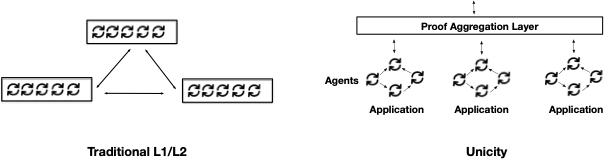
\includegraphics[width=\textwidth]{Comparison.png}
    \caption{A different approach}
    \label{fig:comp}
\end{figure}

Unicity somewhat resembles a (zero transaction) L1 and a set of dynamically spawned L2s, one per contract (agent). Agent instances perform local transaction ordering, obtain a unicity proof and synchronize state with other agent instances. There is always an ``interested party'' (players in a game, owners of tokens) to ensure verifiability and availability. For example consider a simple turn-based game played by three players. There are only three interested parties. To run this game on-chain either in an L1 or an L2 would be highly inefficient, as all the validators would need to execute the game (and all other games) as part of the consensus process. The Unicity approach would be to define the game logic as an agent template with the three players running agent instances. At each turn the player agent instance would update its state, generate a Unicity proof and synchronize with other agent instances.



 A more fundamental example would be digital cash or agents as fungible currency tokens. In this case, for each token there is a single interested party (whoever has ownership of the token). Whenever two parties wish to transact the sender will update ownership of the token to the recipient, generate a Unicity proof and synchronize its state with a new agent instance created by the recipient. At this point the sender is no longer an interested party.


\section{Implementation: Consensus Layer}

The public blockchain is used both as the trust anchor and as the native currency of the system (for compensating network participants and paying of transaction fees). The blockchain is purpose-built for Unicity as a Proof of Work chain similar to Bitcoin with a few modifications.

\begin{figure}[htbp]
    \centering
    \includegraphics[width=0.7\textwidth]{Miners.png}
    \caption{Consensus Layer with Proof of Work Trust Anchor}
    \label{fig:miners}
\end{figure}

\begin{itemize}
\setlength{\leftmargin}{1em}
 \item It works on two-minute block times with RandomX ASIC-resistant hashing algorithm.
 \item A subset of miners, based on winning past block rewards, self-select to operate a BFT consensus subnet operating at one-second block times. The BFT subnet implements a finality gadget to periodically ensure settlement finality.
 \item Transactions are restricted to single inputs, enabling the overall ledger to be decomposed into compact individual coin sub-ledgers which can be verified with the same trust assumptions as the full chain.  This allows for the coin sub-ledgers can be extracted from the blockchain and used off-chain, such as for paying transaction fees in the Agent Layer.
\end{itemize}


\subsection{ASIC Resistance and Fair Mining}

Nakamoto's vision for Bitcoin was based on achieving censorship resistance through decentralization, with the idea that anyone with a computer could participate in the network's consensus mechanism through mining. However, the rapid evolution of mining technology, particularly the development of ASICs, introduced an unforeseen challenge to this egalitarian ideal. These machines, designed solely for the purpose of mining, quickly outpaced general-purpose computer hardware in terms of hash rate, leading to a concentration of mining power. The resulting centralization not only deviated from Bitcoin's original decentralized ethos but also introduced potential vulnerabilities to the network, such as increased susceptibility to 51\% attacks and reduced geographical distribution of miners.

In our view Proof of Work is unsurpassed as means to build a fault tolerant censorship resistant network. It ties the security of the system to a physical quantity (energy) and with certain limitations coins can be fairly and transparently distributed. The last years have seen numerous variations of Proof of Stake as a means to provide a proof of uniqueness. However, the distribution of tokens in Proof of Stake is subject to human oversight, leading to potential errors, malfeasance and fraud. Token allocations and airdrops may give the illusion of decentralization, yet the reality can be quite different. There are certainly limitations to Proof of Work such as potential centralization and slow settlement finality, however these limitations can be overcome with modern technologies.

To prevent centralization of mining power new ASIC resistant hash functions have been developed, of which RandomX represents the state of the art, having been battle-tested in Monero, a privacy preserving cryptocurrency, over several years. Unlike Bitcoin's SHA-256 algorithm, RandomX is designed to be ASIC-resistant and CPU-friendly, leveling the playing field and helping maintain a decentralized network of miners. This democratization not only improves network security through wider participation but also upholds the original Bitcoin vision as a decentralized financial system accessible to all. RandomX works by generating random code for each mining round, including a variety of CPU instructions, memory-hard operations and random code execution that can be efficiently performed by general-purpose processors but challenging to optimize in hardware. This ensures that CPUs remain competitive in mining, preserving the network's decentralization and resistance to the concentration of mining power.




\subsection{Ledger Decomposition}


A simple but key innovation in the Consensus Layer is to restrict UTXOs to single inputs.

\begin{minipage}{\linewidth}
\begin{lstlisting}[language=C++]
if (tx.vin.size() != 1)
    return state.Invalid(TxValidationResult::TX_CONSENSUS,
                         "bad-txns-too-many-inputs",
                         "Transactions must have exactly one input");
\end{lstlisting}
\end{minipage}

Due to the restriction on inputs it is possible to extract a compact single coin sub-ledger from the ledger and transfer it to the Agent Layer for programmability, scalability and privacy.

\begin{figure}[H]
    \centering
    \includegraphics[width=0.8\textwidth]{CoinLedger.png}
    \caption{Decomposition into coin sub-ledgers}
    \label{fig:coinledger}
\end{figure}


Coin splits (not shown in the diagram above) are allowed as they do break the local verifiability, i.e., the verifiability of a single coin depends only on the history of that coin and not the rest of the ledger.


\section{Implementation: Proof Aggregation Layer}

The Proof Aggregation Layer can be explained in terms of the workflow for an agent to agent interaction.

\begin{figure}[H]
    \centering
    \includegraphics[width=0.6\textwidth]{Workflow.png}
    \caption{Agent to Agent Interaction}
    \label{fig:Workflow}
\end{figure}


An agent will execute locally and send a state transition request to the Aggregation Layer. The Aggregation Layer will generate a Unicity Proof i.e., a proof that shows the state transition is unique, and return it to the agent who then synchronizes its state with a recipient agent who can verify both the correctness of the agent computation and the uniqueness of the state history.



\begin{figure}[htbp]
    \centering
    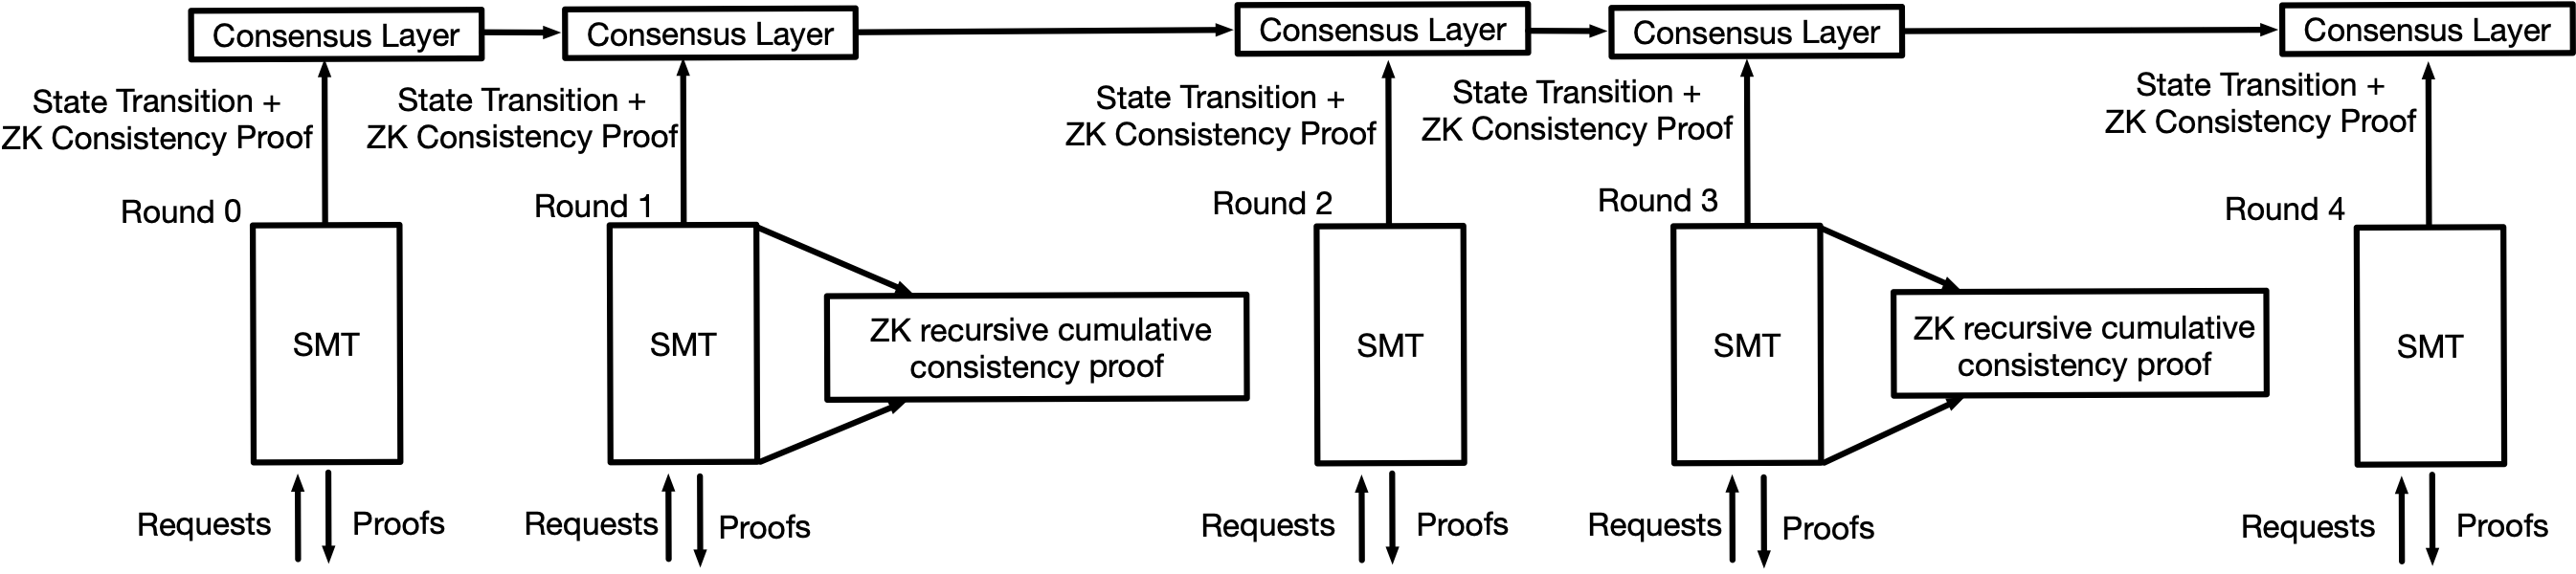
\includegraphics[width=1\textwidth]{SMT-Infra2.png}
    \caption{Proof Aggregation Layer}
    \label{fig:SMT}
\end{figure}


 A Sparse Merkle Tree (SMT) is used such that each unique state transition request from the agent layer is allocated a leaf node in the tree. The details of the request will be described in the next section. The SMT is updated in rounds with a batch of state transition requests per round. In each round the SMT state root is calculated, a ZK SMT consistency proof\footnote{The ZK consistency proof proves that no recorded state transitions were modified or removed during the round.} generated and the SMT state transition (previous SMT state root, new SMT state root, ZK SMT consistency proof) is passed to the Consensus Layer. The validators in the Consensus Layer verify the ZK SMT consistency proof and the validity of request, and then commit to the new SMT root and return a certificate, or cryptographic proof of acceptance of the valid change. After that only requests from the SMT which update the new state root can be accepted.\footnote{The design of the SMT is optimized for ZK proving techniques. Batches of up to 10,000 state transitions can be proven per second using the Poseidon2 hash function, a custom Algebraic Intermediate Representation and Plonky3's FRI STARK prover.}
 
 
 
  A Unicity Proof consists of several elements:

\begin{itemize}
    \item ZK recursively generated cumulative proof at previous ZK checkpoint (common to all requests)
    \item hash-based proof of non-inclusion (the SMT hash chain from leaf to root) for all SMT rounds since the previous ZK checkpoint up to the previous round.
    \item Proof of inclusion (the SMT hash chain from leaf to root) for the current round.
\end{itemize}



The Aggregation Layer is a decentralized permissionless infrastructure built in a hierarchical manner using smaller size SMT sub-trees. An Aggregator, or machine that operates a sub-tree is algorithmically assigned a place in the overall infrastructure according to network demand. Aggregators are incentivized to join the network based on transaction fees that are shared across the Aggregator pool. The infrastructure is designed to be highly redundant and parallelizable i.e. the tree can be dynamically sub-divided into subtrees which operate asynchronously in parallel with redundancy provided by multiple Aggregators processing the same sub-tree. Each sub-tree Aggregator uses a ZK Prover Marketplace to generate a ZK consistency Proof for its sub-tree state transitions and periodically a recursively generated cumulative ZK consistency proof proving the correct operation of the Aggregation Layer for the entire history. 


\begin{figure}[htbp]
    \centering
    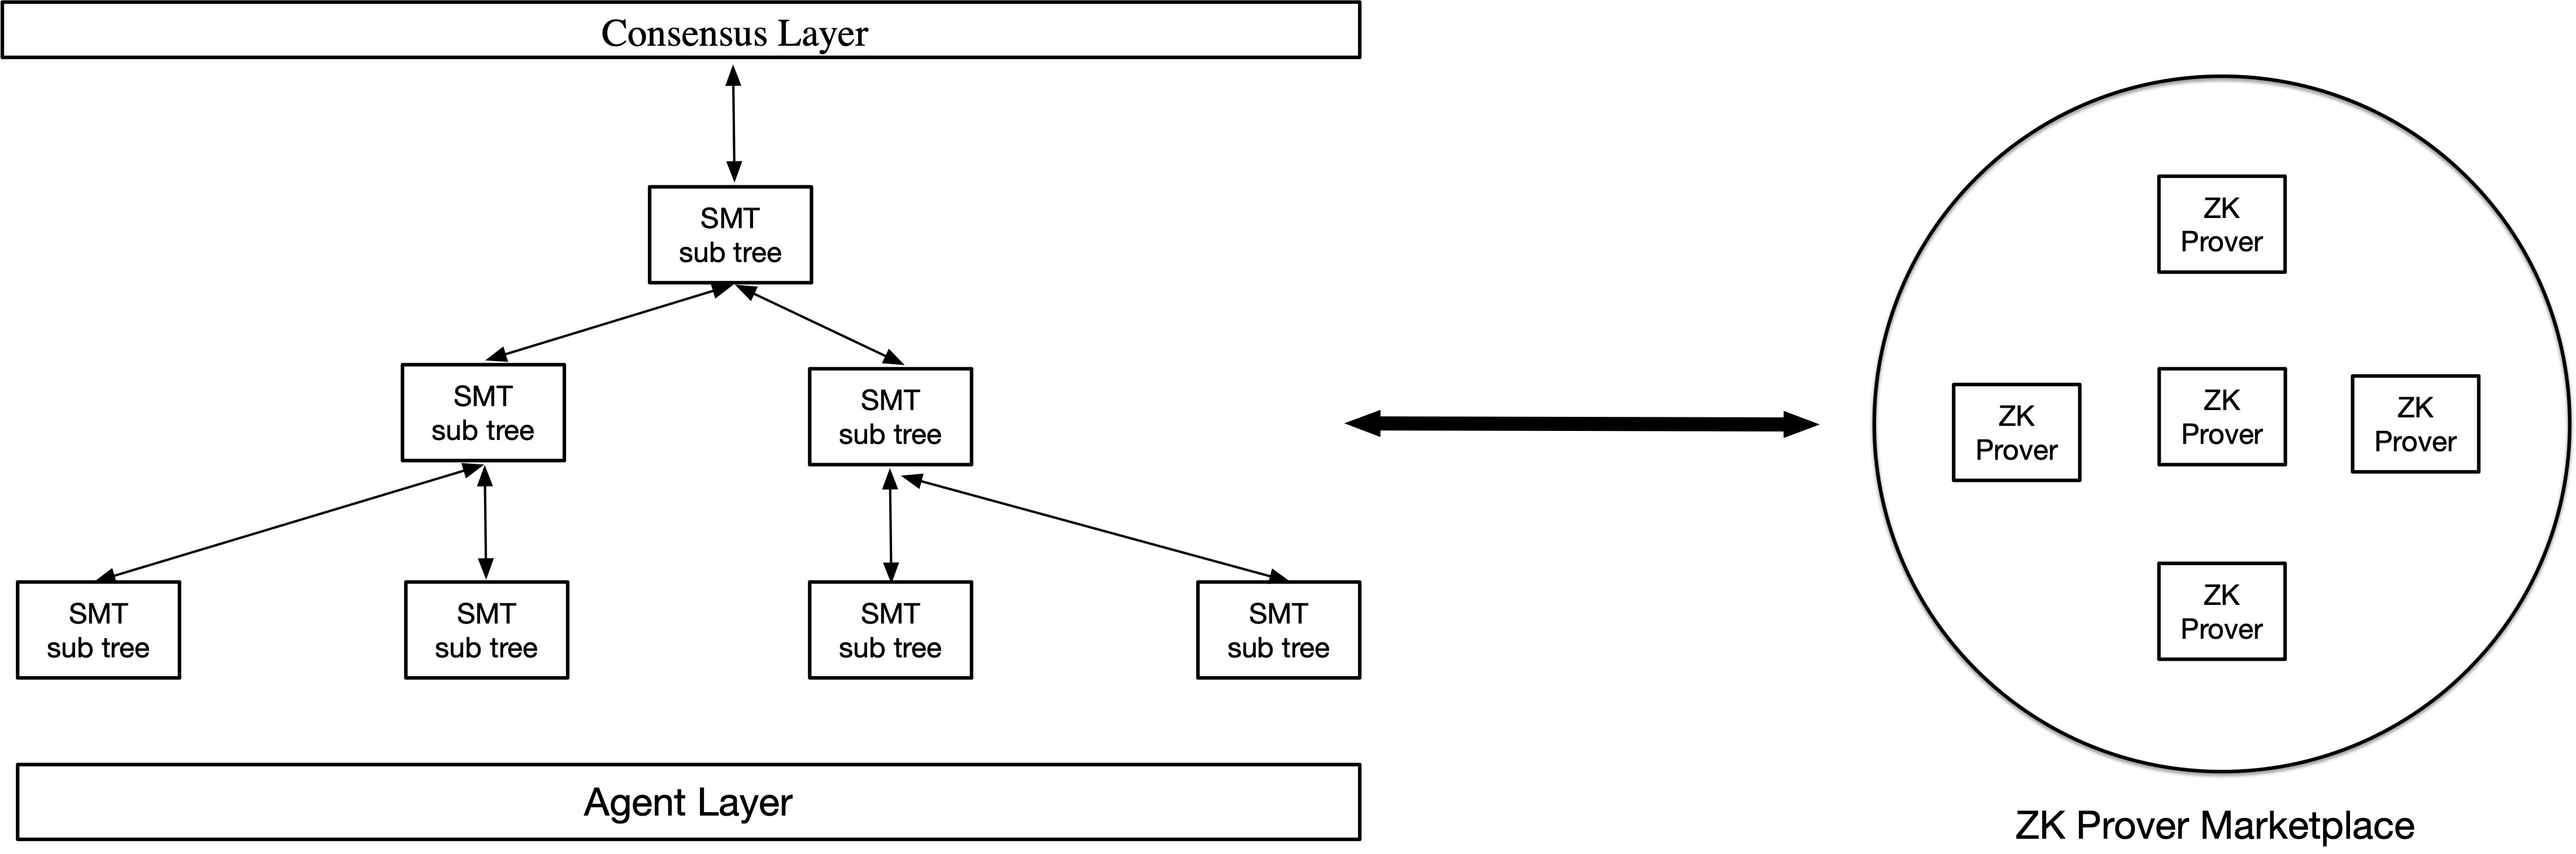
\includegraphics[width=0.9\textwidth]{SMT-ProverMarketPlace.png}
    \caption{Aggregator Hierarchical Infrastructure}
    \label{fig:SMT-Infra}
\end{figure}



\subsection{Dimensioning}

We assume one million state transition requests per second, 256-bit hash values, EC digital signatures, one-second round times and 10-minute ZK checkpoints. We assume that the tree size remains around $32 \cdot 10^{12}$~entries ($10^6$~entries per second with an average lifetime of one year $\approx 32 \cdot 10^6$~seconds) giving a hash-chain size of approximately 1.5\;KB.
A Unicity Proof would be at best case $3$\;KB (just after the ZK checkpoint) and at worst case $900$\;KB (just before the ZK checkpoint).\footnote{The hash-based proof can be discarded after the next ZK checkpoint.}

There is no bottleneck in the system or centralized points of failure. Subtrees operate asynchronously in clusters and their number and location is algorithmically optimized for network conditions.

\section{Implementation: Agent Layer}

The agent layer provides APIs for developers for agent development, agent to agent communication and interfacing with the Unicity Infrastructure for proof generation.

\begin{description}
    \item[Agent:] an encapsulation of code and state that receives inputs from an external environment, executes its code and updates its state and code accordingly.
    \item[Agent instance:] an instantiation of an agent in an execution environment. Multiple execution environments can share the same agent by synchronizing their agent instances.
    \item[Token:] an encapsulation of data that has semantic value.
\end{description}


\subsection{A different programming model}

We will use the example of a Non-Fungible Token (NFT) and highlight the different approach by comparing the operations involved in transferring an NFT in Ethereum and Unicity.  We will assume two users, Alice and Bob. Alice currently owns an NFT and wishes to transfer it to Bob.

In the Ethereum model the NFT exists inside an ERC721 smart contract, executed by the Ethereum Virtual Machine (EVM), the execution environment on the Ethereum Blockchain.



In Unicity the NFT exists inside an agent, instances of which execute locally in their own execution environment(s) (Alice's laptop or mobile device, in the cloud, at the edge or all of the above, simultaneously). Unlike Ethereum ERC721 each NFT is implemented by its own agent.\footnote{A separate agent may act as minting agent, spawning NFT agents.}


In the Ethereum model Alice will send a transaction order to the blockchain network, which will be received by validators, added to a block proposal and then broadcast to the other validators in the network. Alice and Bob can then verify that the transfer took place by checking that the blockchain includes the transaction.


In the Unicity model, Alice will send a transaction order to the agent instance in her execution environment that stores the NFT. The agent instance will then execute the transaction order, request a Unicity Proof from the Unicity infrastructure and synchronize with a new agent instance instantiated in Bob's execution environment. At this point there are identical agent instances in both Alice and Bob's environments. Once synchronized the agent instance in Bob's execution environment will verify both the Unicity Proof (verifying that there are no forks, i.e. Alice is not trying to double spend) as well as the integrity of computation.\footnote{This could be by simply rerunning the agent code or verifying a ZK proof.}

\begin{figure}[htbp]
    \centering
    \includegraphics[width=0.4\textwidth]{UserAgent.png}
    \caption{Unicity User Agent Interaction}
    \label{fig:UserAgent}
\end{figure}

At this point the agent instances can only accept a valid transaction order from Bob to further transfer the NFT. Alice may choose to delete or archive the agent instance that processed the transaction as it can serve no purpose going forward for her.\footnote{Having multiple copies may of course be useful for censorship resistance or fault tolerance depending on the application.}

The major difference in models is the parallelization of compute. There may be an unlimited number of agents all interacting with each other or external parties, and they do not compete for resources on the blockchain. The blockchain still plays a critical role as the trust anchor but does not play a direct role in execution. The model has changed from a sequential to a parallel programming model.

\subsection{State transitions}

The definition of a state transition is agent specific and could be anything from a cryptocurrency transaction, a token mint or player-to-player or agent-to-agent interaction in a multi-player game. In this simple NFT example we use the most basic configuration possible for the purposes of explanatory clarity.

Depending on the application agents may make use of predicates to change their ownership, code or data. Predicates are functions that returns a single TRUE or FALSE, used to check if an input meets certain conditions. Predicates are used in agents to enable customization and programmability. For example the owner predicate is the function that updates the ownership of a agent similar to a Bitcoin unlocking script. The most basic form of an owner predicate would be the verification of a digital signature, i.e., in order to transfer ownership, the signature needs to be signed by a private key that matches the public key stored as part of the predicate.

A data update predicate updates the data field of an agent, a spawn predicate allows an agent to create new agents and a split predicate allows an agent to subdivide into multiple agents which split characteristics of the parent agent (for example an agent that stores a fungible token).

We assume that the current state of the NFT agent consists of:

\begin{itemize}
    \item Alice's address, linked to her Public Key.
    \item An agent ID, created at genesis.
    \item Data, which in the case of an NFT could be an image or a link to an image.
    \item Owner  predicate, this is the unlocking condition i.e. only Alice can unlock the owner predicate and transfer ownership.
\end{itemize}

 Similar to standards such as ERC721, the genesis state and allowable state changes are standardized and encoded in the logic of the agent.

\begin{figure}[htbp]
    \centering
    \includegraphics[width=0.3\textwidth]{CurrentStateAndStateTransition.png}
    \caption{Current State and State Transition}
    \label{fig:CurrentState}
\end{figure}



The first step in the transfer of the NFT to Bob is for Alice to create a state transition. The state transition consists of the hash of the current state and Bob's address.


The second step is for Alice to generate a state transition request, a tuple \{RequestID, Payload, Authenticator\}.

\begin{description}
    \item[RequestID] is the address of Alice concatenated with the hash of the current state.
    \item[Payload] is the hash of the state transition.
    \item [Authenticator] is the digital signature of the payload, signed using Alice’s private key.
\end{description}

The state transition request is then sent to the Unicity Infrastructure where a leaf node is added to the SMT at the address defined by the RequestID and content equal to payload plus authenticator.

\begin{figure}[H]
    \centering
    \includegraphics[width=0.6\textwidth]{STR.png}
    \caption{State Transition Request}
    \label{fig:STR}
\end{figure}

Alice's agent instance will then synchronize its state with Bob's agent instance. To verify that Bob is the new owner the agent instance in Bob's execution environment checks that the state transition is valid and that the Unicity Proof verifies that the state transition is unique. The leaf address of the SMT (the RequestID) is defined by the current state and Alice’s public key only.  Any attempt to double spend would require the generation of an identical leaf node address for which it would be impossible to create a Unicity Proof.

\begin{figure}[H]
    \centering
    \includegraphics[width=0.7\textwidth]{AgentSynchronization.png}
    \caption{Agent Synchronization}
    \label{fig:AgentSynch}
\end{figure}


A critical point is that settlement is local i.e. agents do not depend on the state of other agents to execute. All agents are independent and execute locally in their own environments without referring to the state of other agents. This is in contrast to smart contract platforms such as Ethereum in which smart contracts have full access to other smart contracts' state, as all code and state exists within the memory of a single instance of the Ethereum Virtual Machine. Whilst contracts such as flash loans in Ethereum, i.e., contracts that rely on global state, could be built in Unicity it would defeat the purpose of the parallelization.

\subsection{Analogy with Kubernetes: an agent approach to application deployments}

The Unicity model is a radical departure from traditional blockchain design, allowing massive scale parallelization of agents which interact to execute a decentralized application. An analogy with microservices and Kubernetes is relevant. A microservices architecture involves breaking down an application into small, independent services that can be developed, deployed, and scaled independently, with Kubernetes providing the platform for management and orchestration. The Unicity platform involves breaking down a decentralized application into small independent agents that can be developed, deployed and scaled without a centralized gatekeeper.


\subsection{Zero knowledge: combining verifiable compute and  uniqueness}

As a result of the increased use of blockchain technologies there has been the surge in research and development of Zero Knowledge (ZK) technology. Zcash pioneered the use of zk-SNARKs (Zero-Knowledge Succinct Non-Interactive Argument of Knowledge) in 2016, enabling fully private transactions on a public blockchain. This breakthrough spurred further innovations, such as Ethereum's implementation of zk-rollups for scalability, reducing transaction costs and increasing throughput. As described earlier, Unicity uses ZK extensively at the Proof Aggregation Layer to provide succinct proofs of non-deletion. ZK techniques can also be applied at the Agent Layer enabling agents to provide verifiable proof of computation to other agents.

ZK and Unicity solve different problems that when combined represent a powerful approach to building decentralized applications. ZK provides proof of computation but not proof of uniqueness. Many client side ZK proof generation platforms such a Aztec, ZKSync, Aleo etc. can be used in combination with Unicity to provide proof of computation \textbf{and} proof of uniqueness, effectively moving all compute to the client side and reducing the verification task of a recipient to verifying a single ZK Proof. In the simple example above Bob's agent instance must re-execute the state transition to verify the correctness of computation. If Alice's agent generated a ZK Proof of the state transition, it would reduce the work necessary for Bob's agent instance, and also for future recipients of the NFT to verify the correctness of previous computations.


\section{Programmable Digital Currency}

Bitcoin provided a practical implementation of the ideological commitment to freedom, self-sovereignty, and resistance to government censorship.  It marked a significant advance towards censorship-resistant money with predictable and transparent issuance rules, preventing the kinds of fiscal mismanagement that are inevitable under fiat systems. However, whilst it has proven to be a resilient store of value, it has not seen widespread adoption as a medium of exchange. In this section we show how the Proof of Work coins generated in the Consensus Layer can be extracted and used by agents to provide a highly portable medium of exchange similar to physical cash.

Alice is the owner of a coin - a coin generated through Proof of Work in the Consensus Layer. In order to use it like cash the first step is to transfer the coin to a specified transfer or burn address in the ledger. Alice then creates a new agent with a genesis state defined by the transaction ID of the burn transaction in the ledger. The agent's genesis state includes this transaction ID, the coin sub-ledger, and the genesis ownership predicate. The genesis owner predicate must match the send address in the ultimate transaction in the coin sub-ledger i.e. only the private key that initiated the burn transaction can execute a transfer.

\begin{figure}[htbp]
    \centering
    \includegraphics[width=0.15\textwidth]{CoinGenesis.png}
    \caption{Agent Genesis State}
    \label{fig:GenesisEvent}
\end{figure}

The reason for including the coin sub-ledger is local verifiability. If a recipient had access to a full node of the PoW blockchain they would have the full history and be able to verify the transaction integrity themselves. However, this is quite restrictive and would limit the choices for execution environments. By including the coin sub-ledger a recipient simply needs the genesis block of the PoW blockchain to independently verify the integrity of the coin sub-ledger. The analogy with physical cash is relevant. When someone hands over cash the recipient does not need to verify the integrity of every transaction in history to know that the cash is valid. In other words Unicity agents share the same property of physical cash that verification and settlement happen locally.


When Alice wishes to initiate a transfer she will create a state transition and a state transition request similar to the NFT example above. In this case the token is fungible which means that for a transfer less than the value of the coin the agent will split into two agents, one with the value of the transfer and the other with the value of the remainder.

\begin{figure}[H]
    \centering
    \includegraphics[width=0.9\textwidth]{Alice-Transfer.png}
    \caption{Transfer of a coin minted in the Contract Execution Layer}
    \label{fig:Alice Transfer}
\end{figure}


Bob's agent will verify the integrity of the coin sub-ledger (verifying the burn transaction) as well as the integrity of the state transition and the Unicity Proof. At this point only Bob's agent can execute a transaction order i.e., Bob is now under full control of the agent and therefore the underlying value of the coin.

\section{Decentralized Finance}

There are two compelling reasons for decentralized finance (DeFi). For individuals, the appeal is freedom - the elimination of intermediaries, allowing direct engagement in financial transactions without relying on centralized entities such as banks or payment processors. This provides greater financial autonomy and protection against authoritarian government censorship, ensuring the freedom to transact and access financial services without external control or intervention. For institutions, incorporating elements of DeFi can enhance security and automation by eliminating the need for human oversight. Processes can be streamlined, operational costs reduced, and risks associated with human error or fraud mitigated, while enforcing regulatory compliance at the code level. Whilst these are two very different perspectives, it is clear that DeFi has the potential to revolutionize financial services, driving innovation and empowerment at both the individual and institutional levels.



While significant progress has been made in productizing DeFi and enhancing the user experience, much work remains. Just as no one is currently running Call of Duty or fully self-driving software in a smart contract today, no one is operating the New York Stock Exchange (NYSE) on a smart contract either. The agent-based approach of Unicity offers a potential path forward by breaking down the components of an exchange into independent agents that execute off-chain in parallel.

\begin{figure}[H]
    \centering
    \includegraphics[width=0.7\textwidth]{ABEX.png}
    \caption{Agent-Based Decentralized Exchange}
    \label{fig:ABEX}
\end{figure}


Figure \ref{fig:ABEX} shows a simplistic view of a decentralized exchange built using a set of interacting agents. The core agents are the Central Limit Order Book (CLOB) agents which manage individual trading pairs. Depending on requirements these can be deployed and replicated on consumer laptops for a fully permissionless censorship resistant network, or operating in high-powered servers in high availability data centers. From a functional perspective, the end result is the same. Individual agents execute in parallel, and synchronize state in a fully transparent, verifiable, and autonomous way. Other agents provide KYC access, margin management, act as price oracles and provide any other functionality that is required to operate the exchange.


\section{Decentralized Gaming}

Although blockchain technology has been proposed as a means of enhancing transparency and facilitating value exchange in gaming, its current application has largely been limited to asset tokenization within centralized game architectures. Due to the limitations of existing designs, using blockchain for actual game execution remains impractical. However, the potential benefits of decentralized gaming are clear: players can gain true ownership of interoperable assets across different games, enjoy transparency and community-driven governance, experience censorship resistance, unlock innovative business models like play-to-earn, and support fair reward systems for creators.


The motivation behind this work came from a desire to solve a real problem in the gaming industry. The industry has, to a large degree, converged on a client-server approach and while the accepted view is that although pure client-side execution of multi-player games is technically possible, it considered impractical due to issues of security and synchronization. However, the client-server approach is itself severely limited as it is technically challenging to have many players interact in real-time on the same server instance. Modern simulations are limited to a few hundred players interacting in the same shared world due to this limitation.


Unicity is an attempt to overcome these limitations and build a truly decentralized game engine for massive online multi-player immersive simulations. In this case decentralization is not a “nice to have” but an essential requirement to allow complex multi-player interactions with potentially millions of players all interacting online. Moving execution to the client side would allow the system to scale, with blockchain technology providing a security layer that guarantees honest gameplay.


A user will initialize the game environment and interact with a set of agents that execute the game mechanics such as NPCs, real-world assets and in-game assets. As users interact with the virtual world and approach other players, the players' agents will synchronize with each other with verifiable state transitions proving that the game logic has been followed and enabling game synchronization and exchange of assets.

\begin{figure}[H]
    \centering
    \includegraphics[width=0.5\textwidth]{game.png}
    \caption{Three player simulation}
    \label{fig:game}
\end{figure}

In the event of a failed verification action can be taken defined by the game logic, such as rewinding the game to the previous known good state. In this way, a completely new type of game engine can be built with the game components consisting of either autonomous agents, managing game logic, and semi-autonomous agents operating on behalf of the player, and interacting with the environment and other players.

\section{Decentralized AI}



The pace of AI advancement in recent years has been nothing short of breathtaking. From the remarkable performance of Large Language Models (LLMs) to AI systems capable of complex problem-solving and creative tasks, the capabilities of artificial intelligence are expanding exponentially. This rapid progress, while promising to accelerate further, also raises significant concerns about potential risks and unintended consequences of unchecked AI development. As AI systems become more sophisticated and autonomous, there is an urgent need to implement robust guardrails to ensure these powerful technologies remain aligned with human values and societal well-being. However, a world increasingly reliant on AI's probabilistic and often unexplainable models, as opposed to deterministic processes, makes it extremely challenging to implement these guardrails and verify alignment with society's goals and values.



Blockchain technology has been proposed as a means to build transparent and immutable AI systems. However, due to the limited processing power, high latency, and costly nature of on-chain operations, it is impractical to execute complex AI models directly on-chain. The size of AI models far exceeds the storage capabilities of most blockchain platforms, and the slow transaction speeds along with high costs make real-time AI decision-making virtually impossible in a purely on-chain environment. Unicity overcomes these obstacles to the convergence of AI and blockchain technology. Execution happens at native speed off-chain in AI agents' local environments but with the same security guarantees as if agents were executing on-chain. The platform enables the building of verifiable AI systems that allow human operators and agents to interact through trustless state verification, deterministically verifying that execution has been carried out in accordance with agreed rules, and taking action when they do not.


\begin{figure}[H]
    \centering
    \includegraphics[width=0.5\textwidth]{AI.png}
    \caption{Agents coordinating on a task through trustless state verification }
    \label{fig:ai}
\end{figure}



When combined with a native currency as a means to reward agents based on their performance, contributions, or desired behavior, Unicity lays the foundations for a fully secure and verifiable decentralized ecosystem. AI agents can be programmed to earn digital currency for completing tasks, solving problems, or contributing computational resources. This currency acts as the medium of exchange in an agent economy, driving collaboration and competition among AI agents, motivating them to optimize their actions for efficiency and productivity.


The incentive structure  enables the creation of decentralized marketplaces where AI agents can exchange data, services, or computational power with other agents or human participants. Digital currency provides a transparent, automated way to measure the value of contributions, ensuring that autonomous AI systems remain aligned with predefined goals and facilitating verifiability between agents, human operators, and stakeholders. The structure promotes self-sustaining, scalable systems where AI agents evolve and improve autonomously while being rewarded for their beneficial outputs. By addressing the challenges of on-chain AI execution and providing a framework for verifiable, incentivized AI agents, Unicity paves the way for a new era of decentralized artificial intelligence that balances innovation with accountability and alignment with human values.


\end{document}
